\scanpage{11}
\uline{Variantes} \unsure{débarrassées|débarrassés} d'hypothèses noethériennes\ldots

\uline{Variante} Pour un morphisme $Y\longrightarrow X$ \uline{non ramifié}

\uline{N.B.} Il faudrait également \uline{moduler} le th. précédent\ldots
\figure{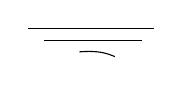
\begin{tikzpicture}[x=1cm,y=1cm]\draw (0,0)--(1.6,0);\draw (.2,-.16)--(1.45,-.16);\draw (.65,-.3)..controls(.9,-.28)and(1,-.32)..(1.1,-.36);\end{tikzpicture}}

\uline{Théorème} Soit $f:X-S$ morphisme de type fini, $S$ loc. noeth., $E$ cohérent sur $X$. Soit $F$ sur $S$ le \unsure{s-foncteur} de $\unsure{S|\underline{S}}$
\[
F(S')=\begin{cases}\varnothing&\text{si }F_{S'}\text{ non plat \inserted{(resp. non fid plat)} sur }S'\\\{\varnothing\}&\text{sinon}\end{cases}
\]
Pour que ce foncteur soit représentable, il \unsure{f.s.} qu'il commute aux limites projectives adiques d'anneaux artiniens.

Vérification des divers p\textsuperscript{ts}

1°) Faisceau pour fpqc Clair

2°) Commute aux $\varinjlim$ d'anneaux : EGA $\unsure{IV}$ 8 et $\unsure{IV}$ 11
\margin{$\times$ type fini \unsure{seul}, $F$ coh}

3°) Condition de commutation aux $\varprojlim$ d'artiniens

4°) 5°) 6°) Si $A\unsure{-|\to}A'$ injectif ($A'$ fini sur $A$ local artinien) alors $F(A)\longrightarrow F(A')$ bijectif i.e. $F(A')\ne\varnothing\Rightarrow F(A)\ne\varnothing$ i.e. $X_{A'}$ plat (fid plat) sur $A'\Rightarrow X_A$ plat (fid plat) sur $A$ EGA IV 11

7°) --- $F(T_0)\ne\varnothing$, $F(U)\ne\varnothing\Rightarrow F(T)\ne\varnothing$ i.e. $X_{T_0}$ plat et $X_U$ plat $\Rightarrow X_T$ plat EGA IV 11.
\mspage{10}
